\documentclass{beamer}
\usepackage{amsmath,amssymb}
\usepackage{graphicx}
\usetheme{Warsaw}
\usecolortheme{beaver}
\usetheme[pageofpages=of,% String used between the current page and the
                         % total page count.
          bullet=circle,% Use circles instead of squares for bullets.
          titleline=true,% Show a line below the frame title.
          alternativetitlepage=true,% Use the fancy title page.
          titlepagelogo=../pict/lambang-its-bw-std,% Logo for the first page.
          ]{Torino}

\author{Mifta Nur Farid\\Dhany Arifianto}
\title{\huge Speech Segregation Based-on Binaural Cue: Interaural Time Difference (ITD) and Interaural Level Difference (ILD)}
\institute{VibrasticLab\\ Dept. of Engineering Physics ITS}
\date{August 23, 2016}

\begin{document}
% DO NOT COMPILE THIS FILE DIRECTLY!
% This is included by the other .tex files.

\begin{frame}[t,plain]
\titlepage
\end{frame}

%\begin{frame}
%\frametitle{Contents}
%\tableofcontents
%\end{frame}

\section{Introduction}
\begin{frame}[t]{Motivation}
\begin{itemize}
\item Hearing loss
\item Cause of hearing loss
	\begin{itemize}
	\item Infection/ injury 17.1\%
	\item Born with hearing loss 4.4\%
	\item Noise damage 33.7\%
	\item Ageing 28\%
	\item Other 16.8\%
	\end{itemize}
\item Hearing loss $\rightarrow$ hearing aids
\item Hearing aids $\rightarrow$ amplify all sounds
\item Most optimal hearing aids: Binaural hearing aids $\sim$ human auditory system
\end{itemize}
\end{frame}

\begin{frame}[t]{Human auditory system}
\begin{itemize}
\item Human auditory ability $\rightarrow$ cocktail party effect
\item Binaural hearing $\rightarrow$ localization $\rightarrow$ segregation
\begin{center}
	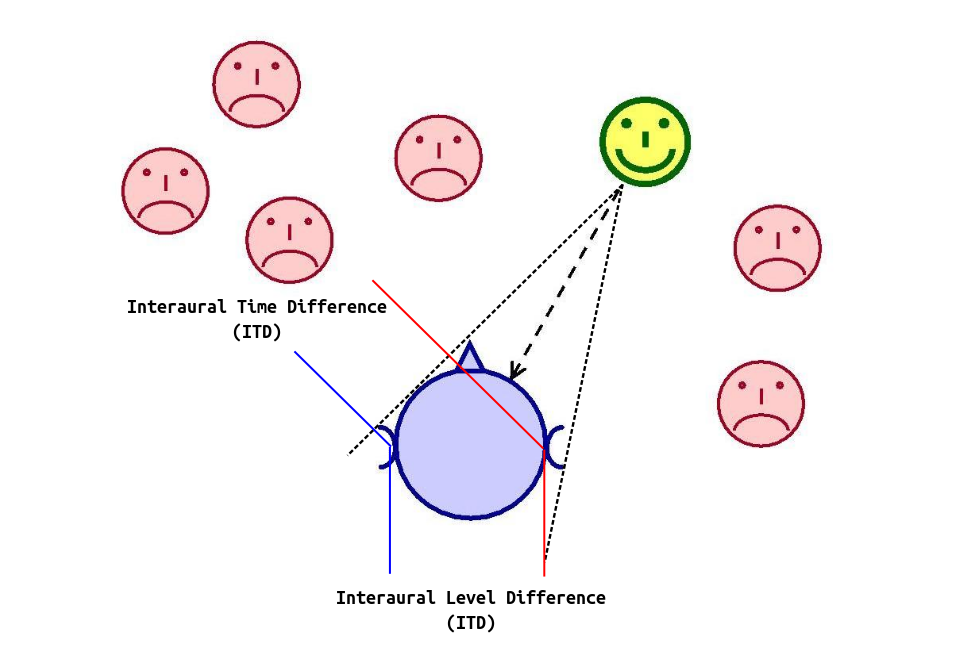
\includegraphics[scale=0.25]{../pict/CPP.png}
\end{center}
\end{itemize}
\end{frame}

\section{Methods}
\begin{frame}[t]{Architecture Model}
\begin{center}
	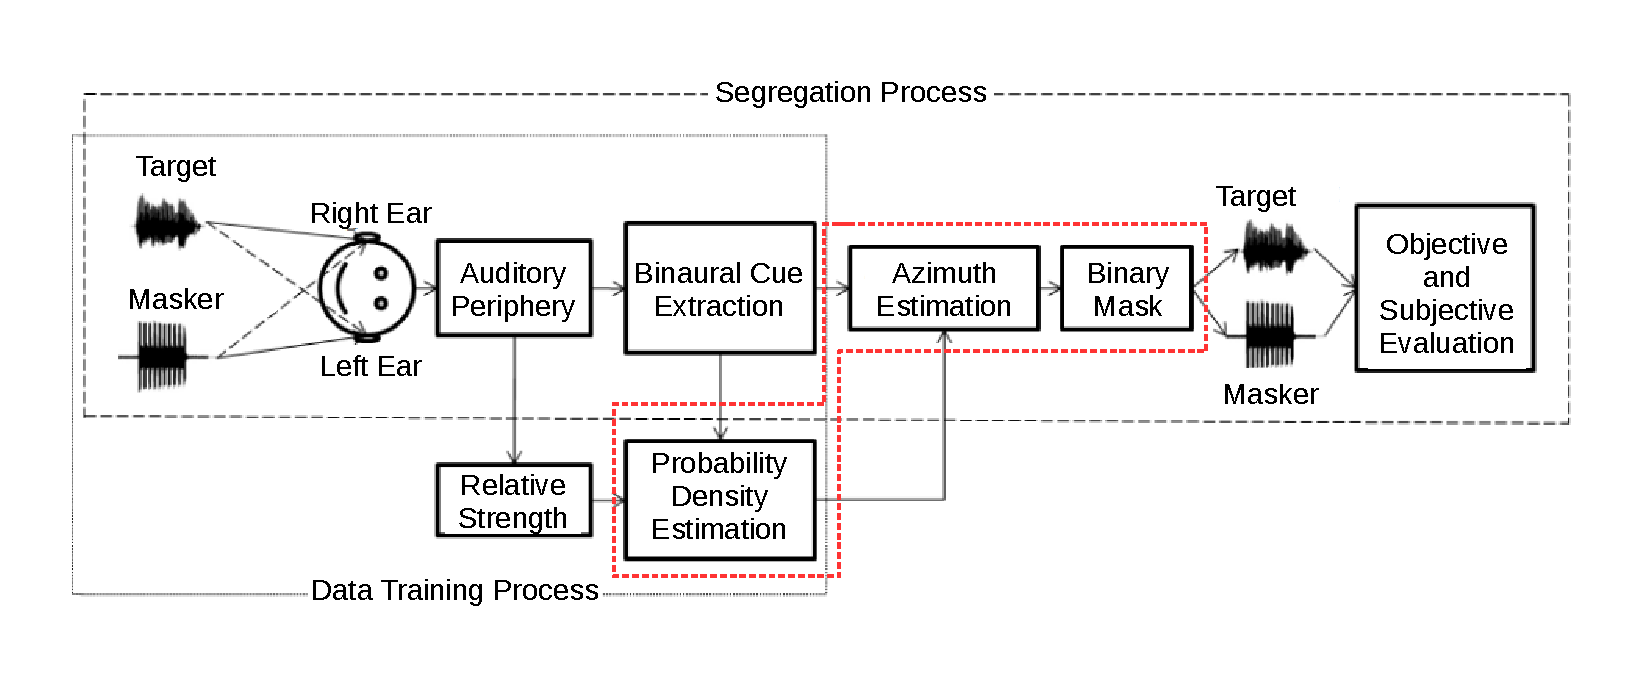
\includegraphics[scale=0.4]{../pict/model_architecture.pdf}
\end{center}
\end{frame}

\begin{frame}[t]{Experiment Setup}
\begin{itemize}
\item Experiment Setup 1 and 2.
\begin{center}
	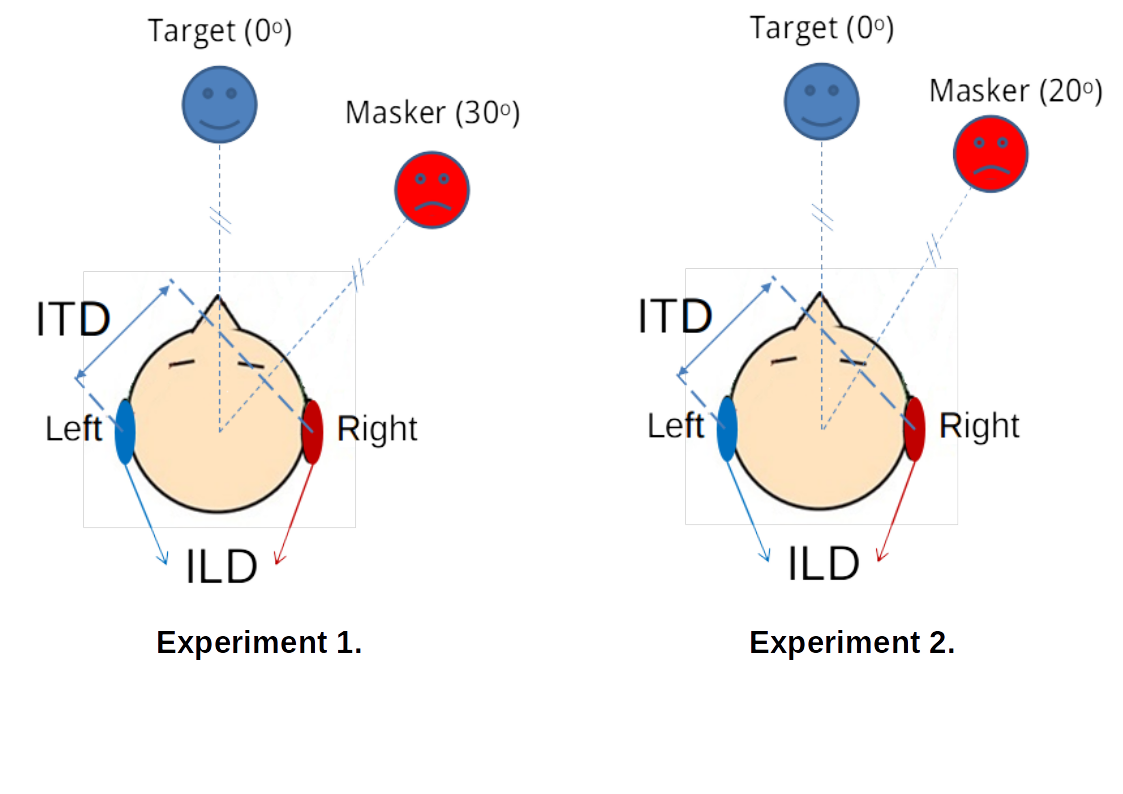
\includegraphics[scale=0.3]{../pict/exp1-2.png}
\end{center}
\end{itemize}
\end{frame}

\begin{frame}[t]{Experiment Setup}
\begin{itemize}
\item Experiment Setup 3 and 4.
\begin{center}
	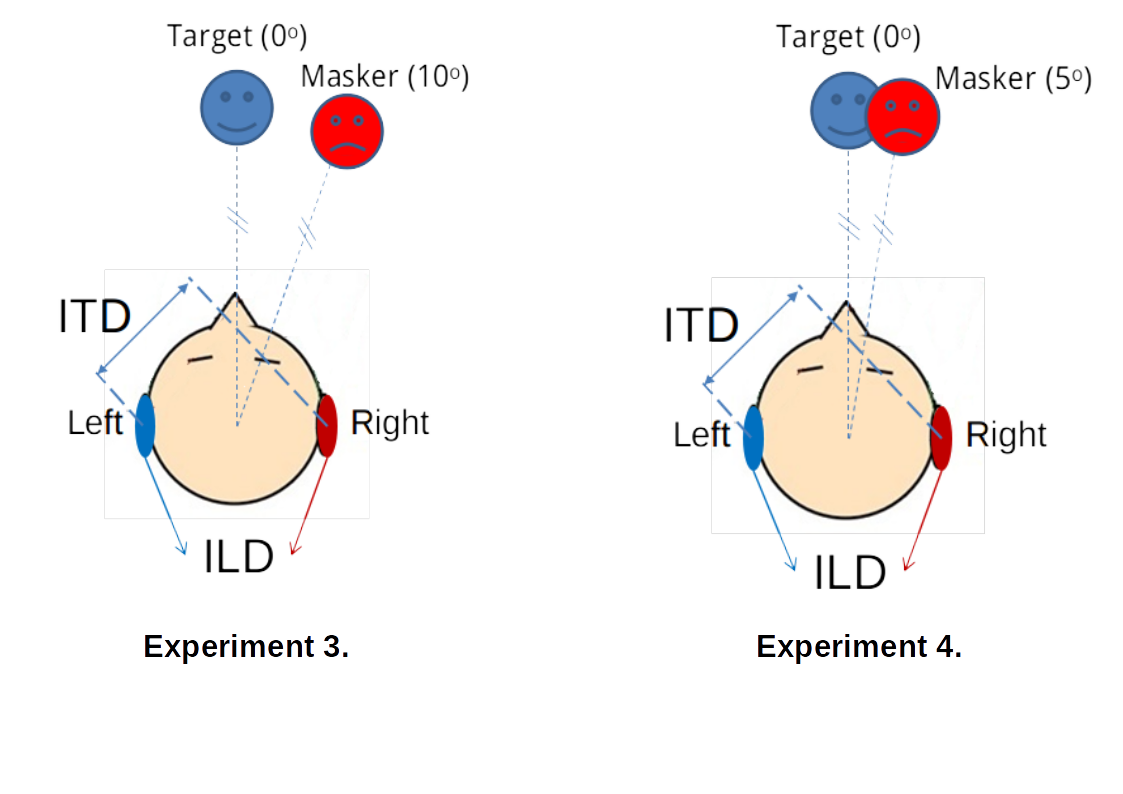
\includegraphics[scale=0.3]{../pict/exp3-4.png}
\end{center}
\end{itemize}
\end{frame}

\begin{frame}[t]{Probability Density Estimation}
\begin{itemize}
\item Experiment setup 1 (SIR 10 dB, 500 Hz)
\end{itemize}
	\begin{center}
	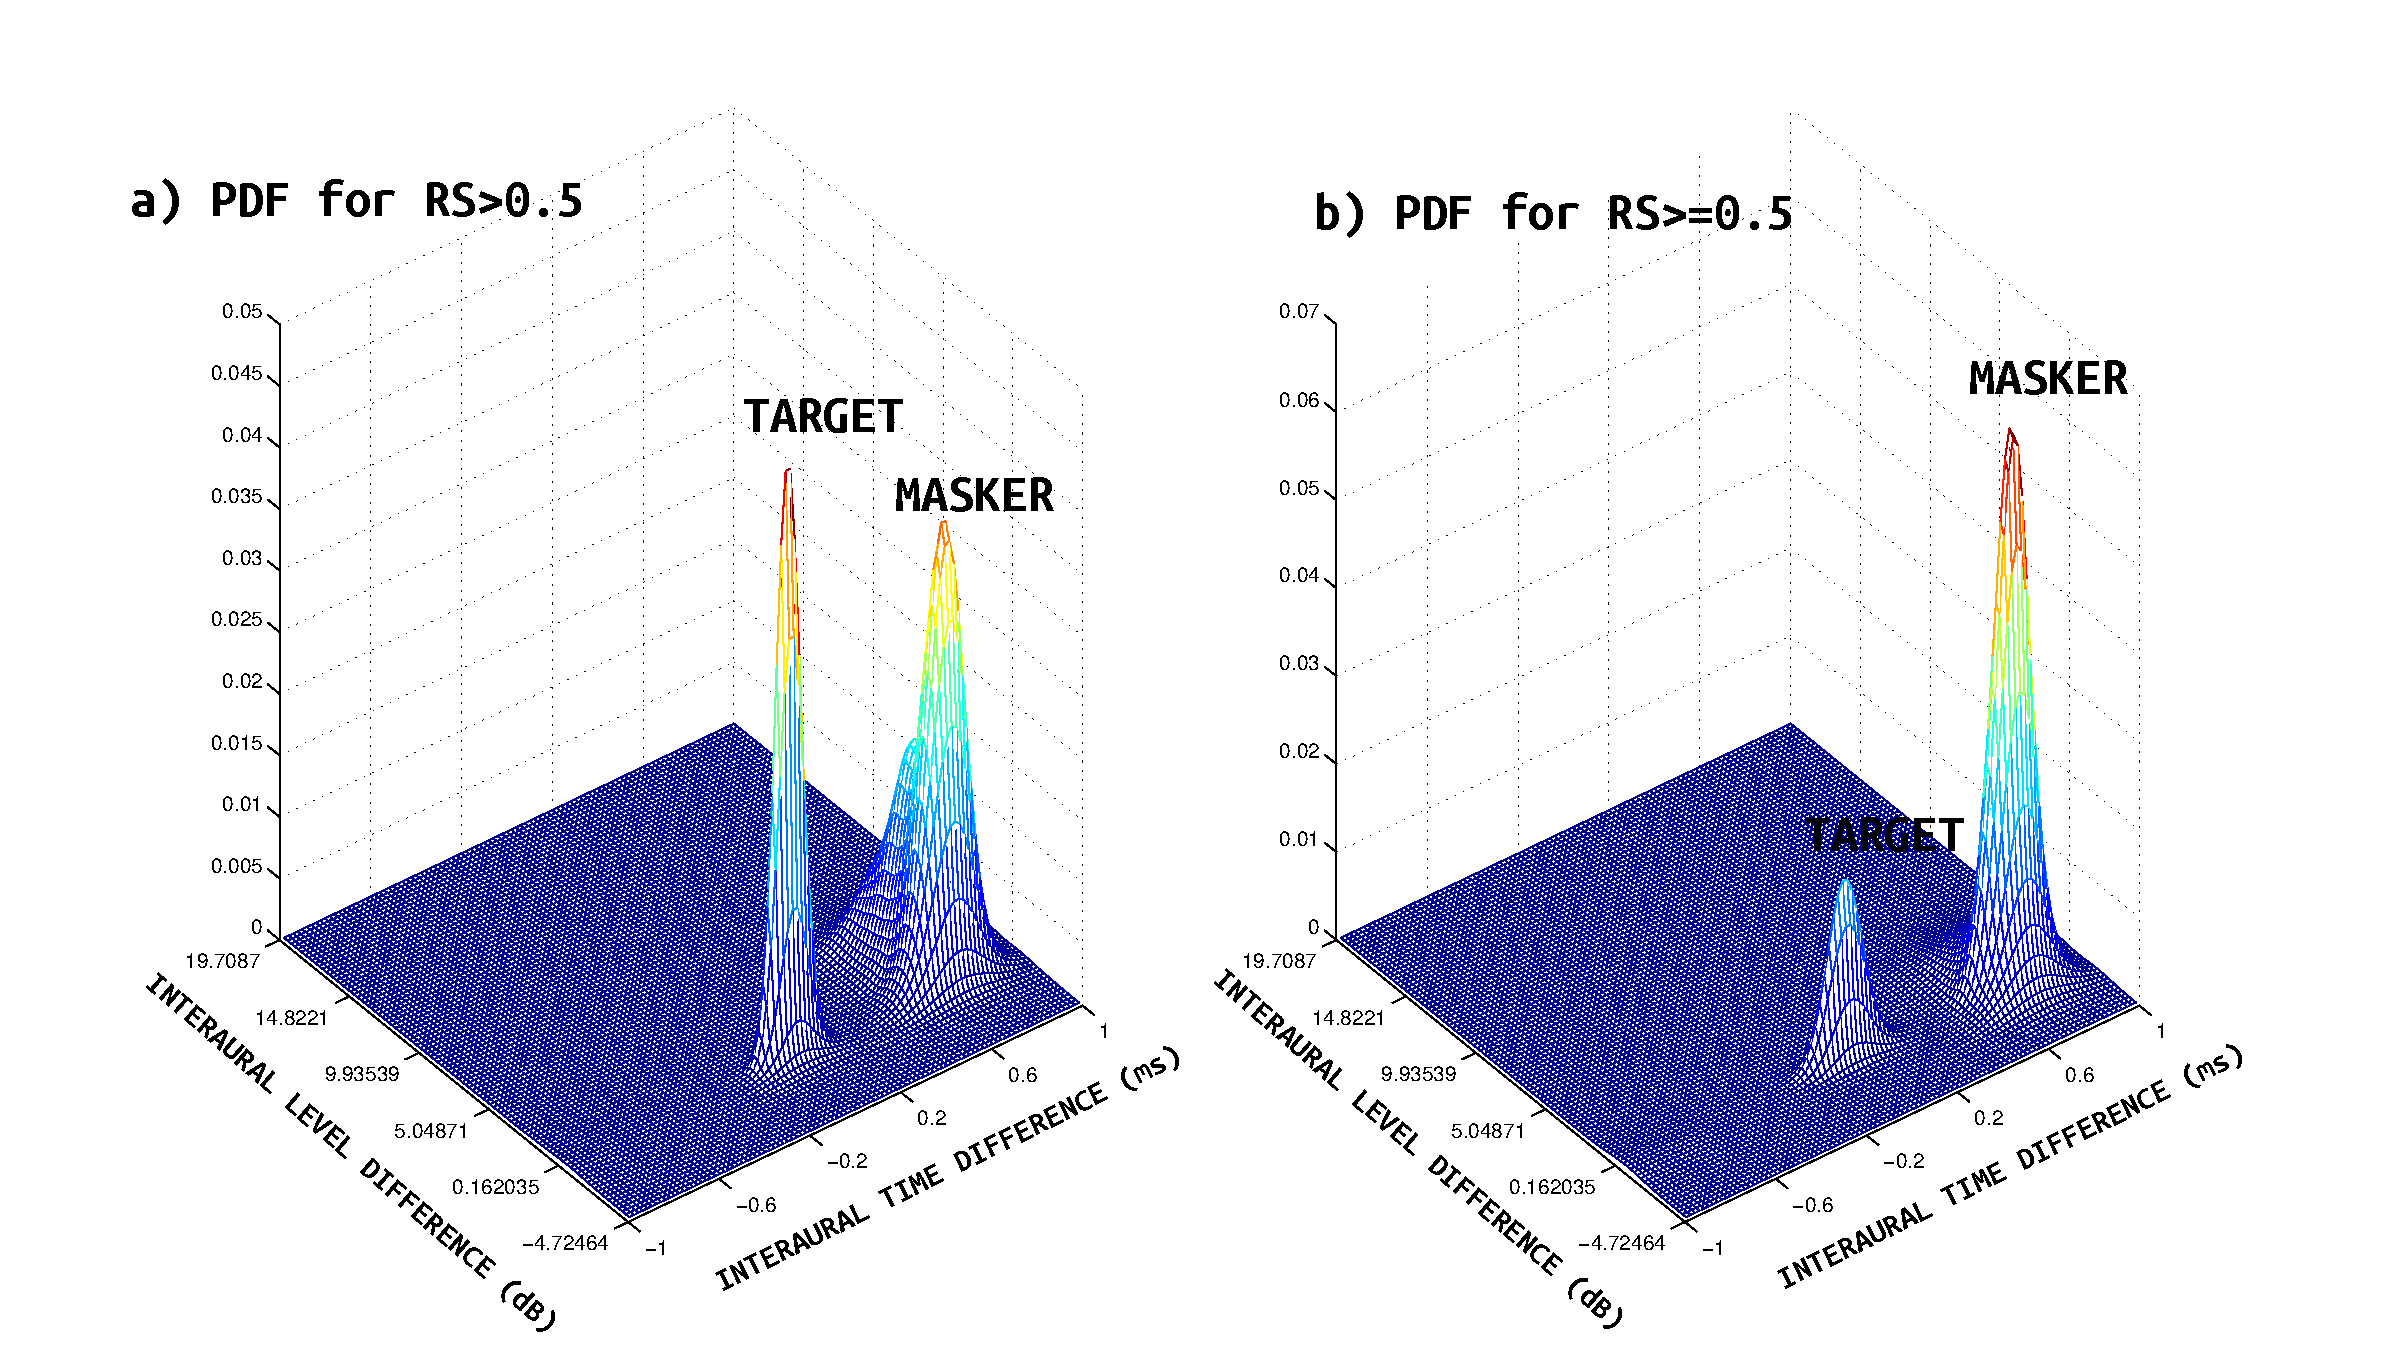
\includegraphics[scale=0.27]{../pict/plot_probability_T0MM30FP10_500Hz.pdf}
	\end{center}
\end{frame}

\begin{frame}[t]{Azimuth Estimation}
\begin{itemize}
\item Experiment setup 1 (SIR 10 dB, 500 Hz)
\begin{equation}
{\scriptstyle C(i, j, \tau) ~=~ \frac{\sum_{k=0}^{K-1}(l_i(j-k)-\bar{l_i})(r_i(j-k-\tau)-\bar{r_i})}{\sqrt{\sum_{k=0}^{K-1}(l_i(j-k)-\bar{l_i})^2}\sqrt{\sum_{k=0}^{K-1}(r_i(j-k)-\bar{r_i})^2}}}
\end{equation}
\begin{center}
    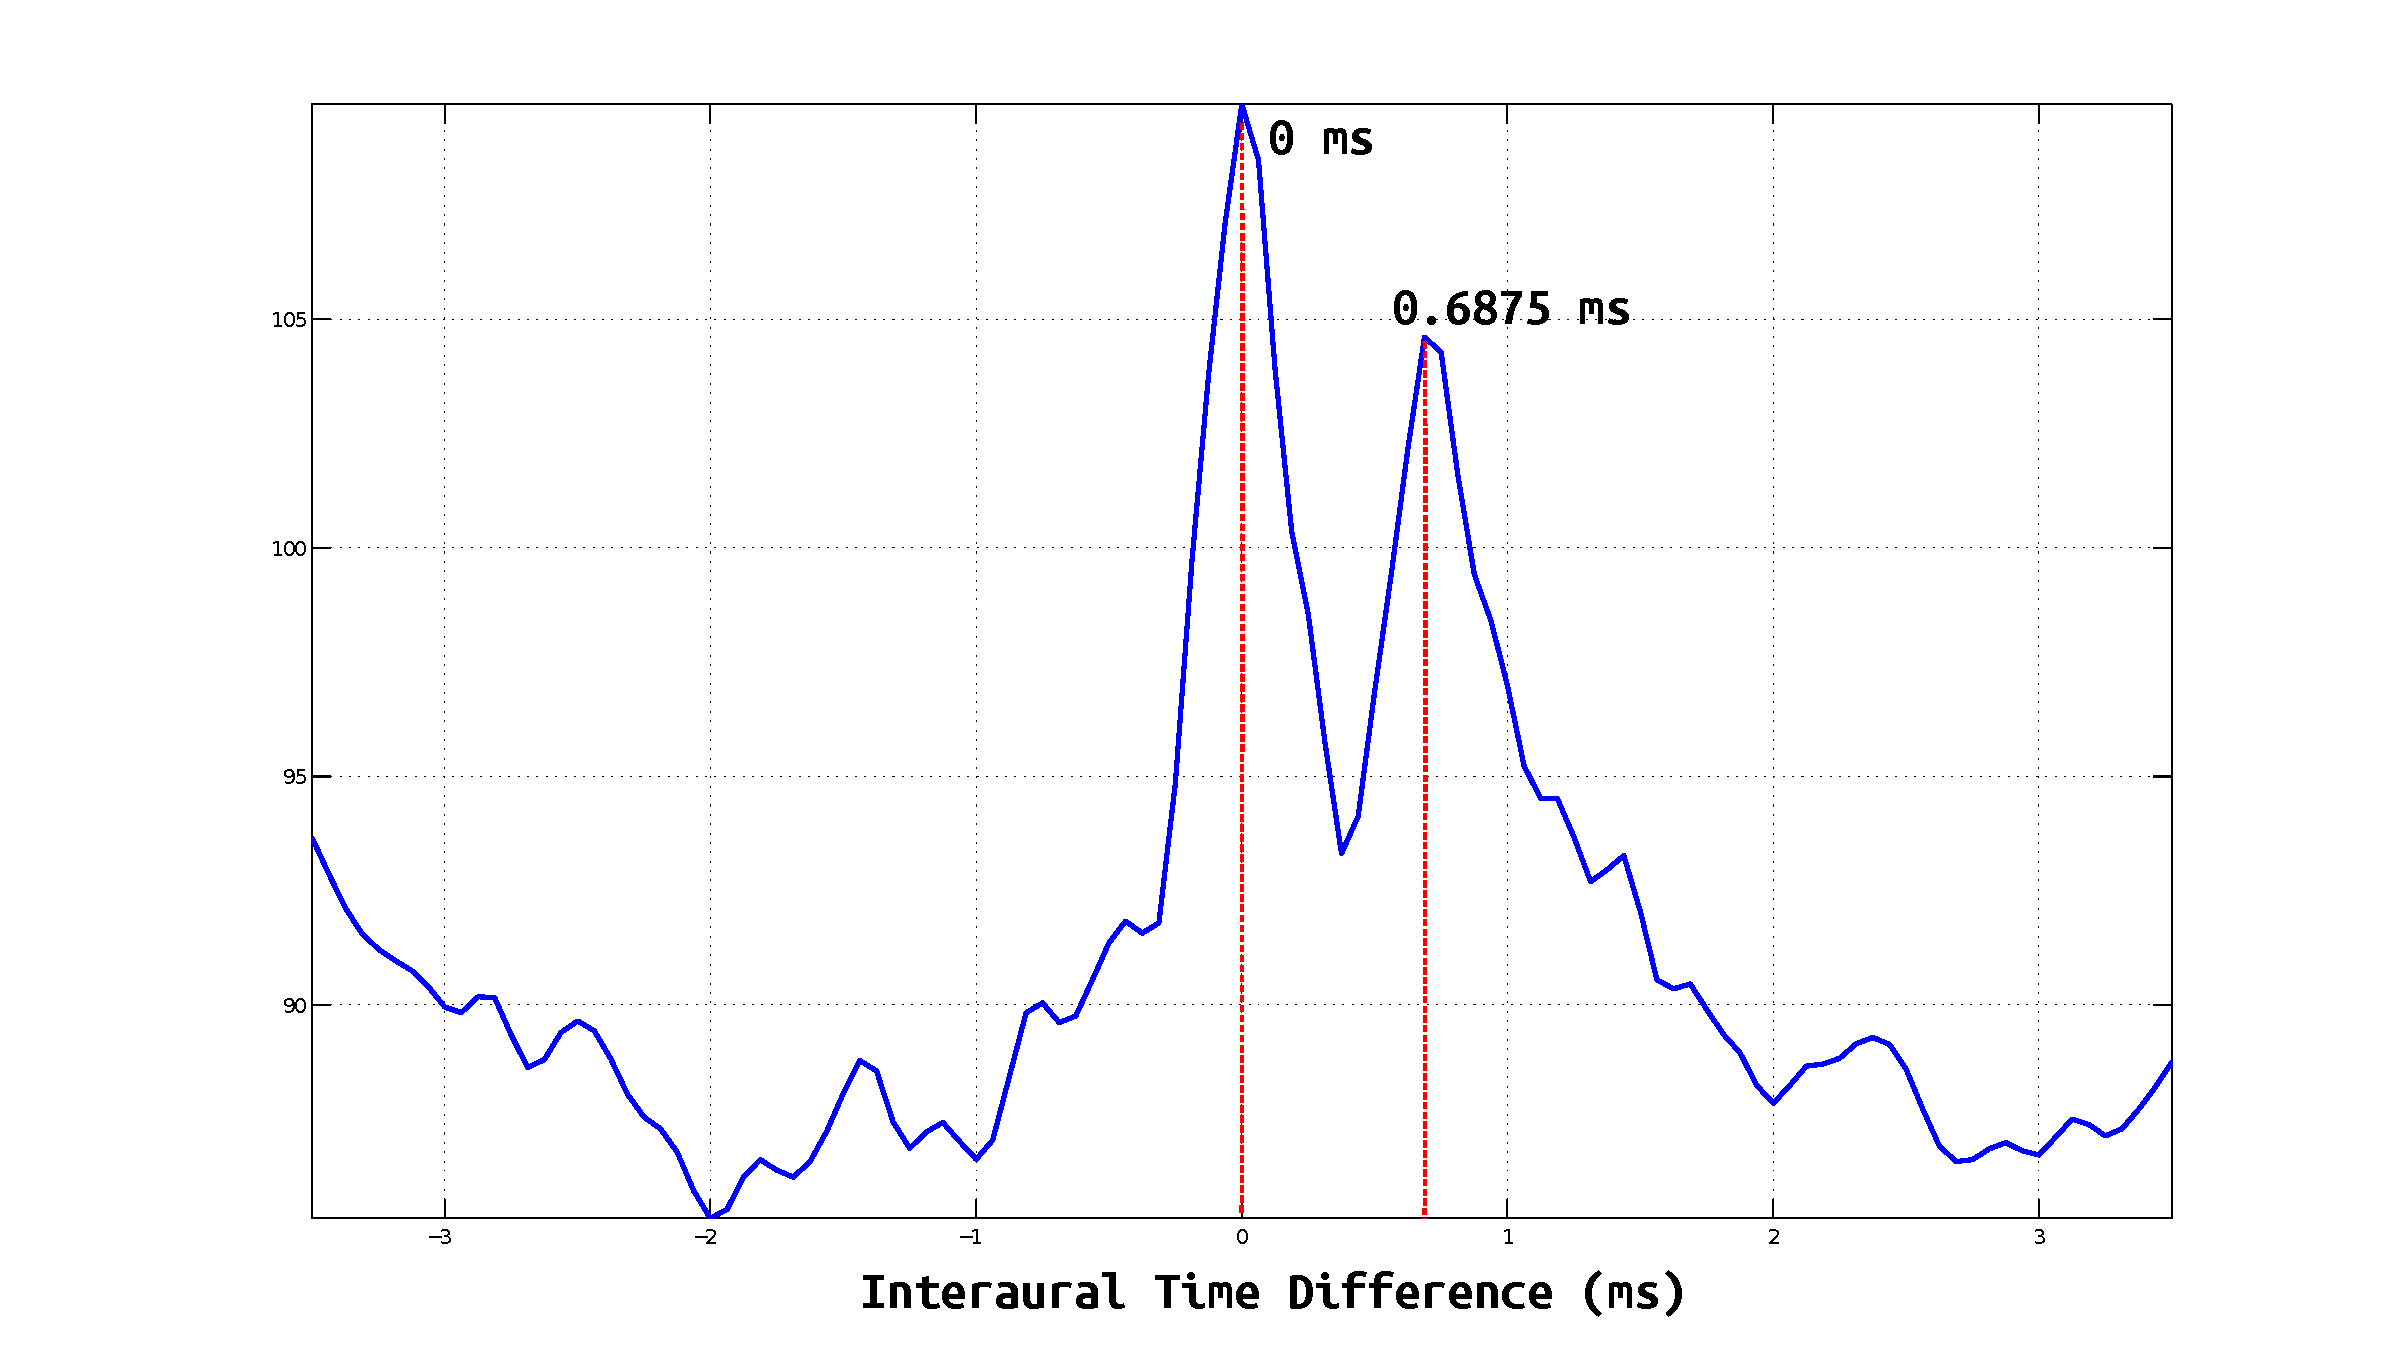
\includegraphics[scale=0.2]{../pict/azimuth.pdf}
\end{center}
\end{itemize}
\end{frame}

\begin{frame}[t]{Binary mask estimation}
\begin{itemize}
\item From both binaural cue (ITD and ILD), binary mask can be estimated using
\begin{equation}
BM =
    \begin{cases}
      1, & \text{if}\ \{(PDE~RS > 0.5) > (PDE~RS \leq 0.5)\}\\
      0, & \text{otherwise}
    \end{cases}
\end{equation}
\end{itemize}
\end{frame}

\section{Results}
\begin{frame}[t]{Results}
Comparison of spectrum and waveform between mixtured, clean and estimated signal
    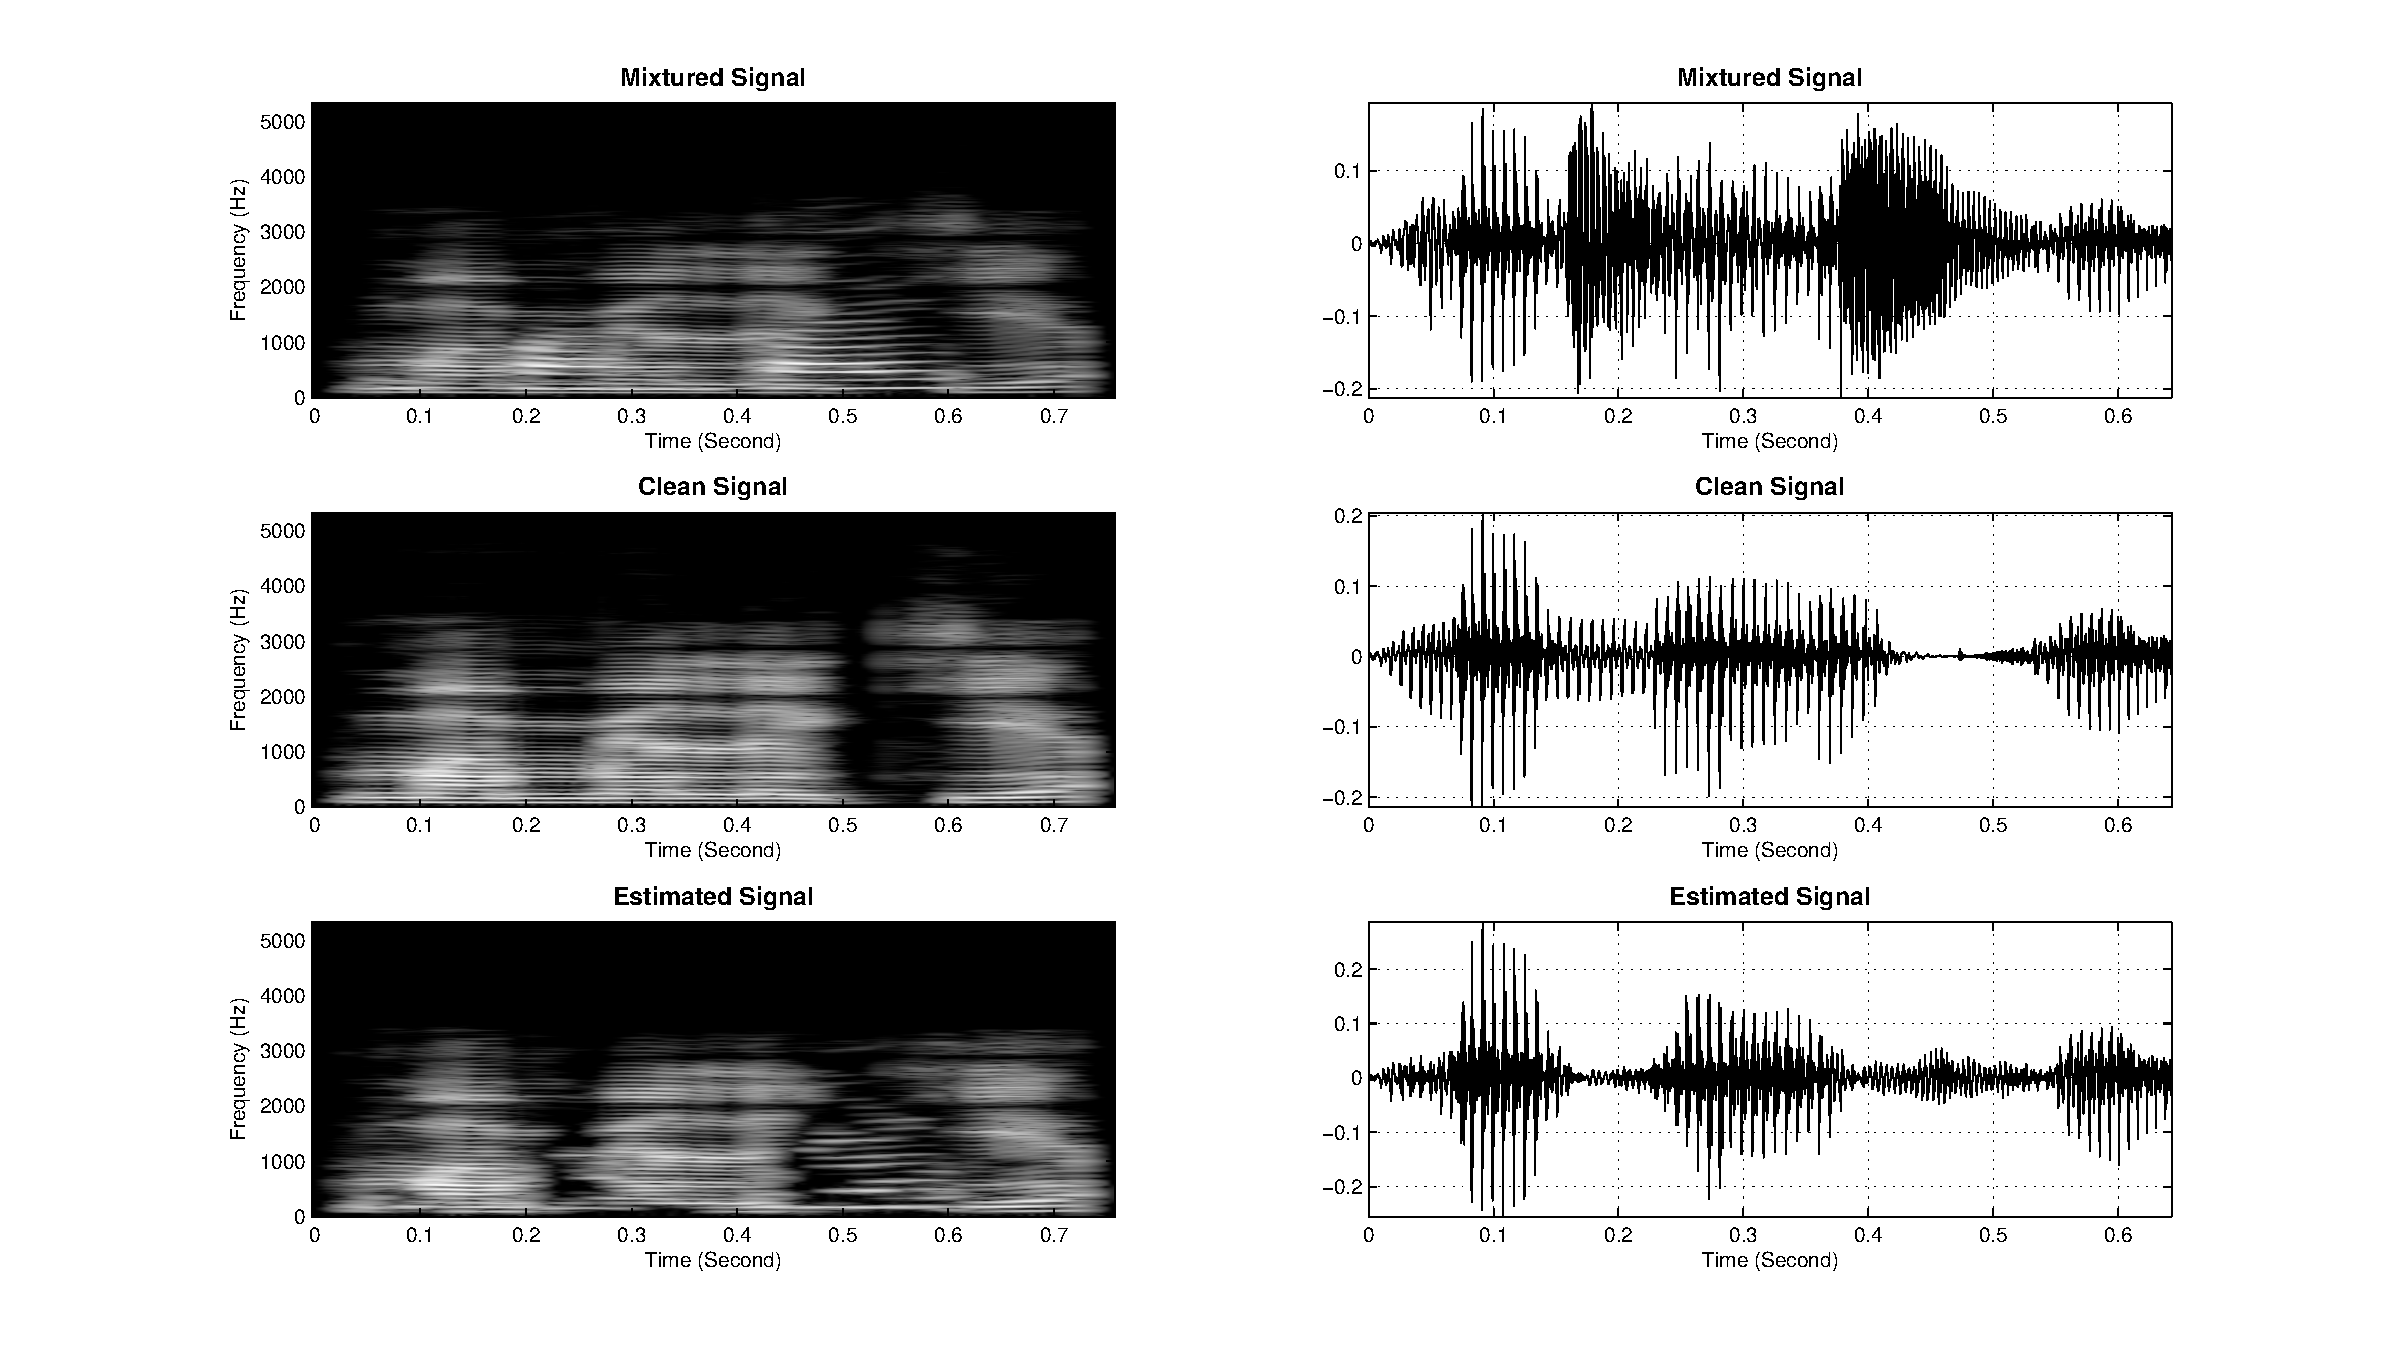
\includegraphics[scale=0.27]{../pict/spectro07.pdf}
\end{frame}

\begin{frame}[t]{Subjective Evaluation}
%The database used Indonesian voice which amounts to 5-8 words per sentence. This database was recorded at anechoic room so there is no reverberation on database. There are two types of sound, there are male voices and female voices. Respondents are 18-23 years old that selected so that it is assumed to have good hearing. Testing is done at anechoic room so that the respondent is not disturbed another voices when listening to stimuli [12]. Headphone that used is Sennheiser HD 650. Entire stimuli (520 sencences) tested to 10 respondents. The task of the respondent is listen stimuli without repetition and then repeated that stimuli by typing, writing, or saying and then typed by the other [1].
\begin{itemize}
\item Percent correct words
\begin{itemize}
	\item Ten respondents: 18 - 23 years old, have good hearing.
	\item Testing is done at anechoic room.
	\item 520 sentences stimuli, each sentece contain 4 - 8 words
	\item The task of the respondent is listen stimuli without repetition and then repeated that stimuli by writing.
	\item How many percent word is correct for entire words.
\end{itemize}
\end{itemize}
\end{frame}

\begin{frame}[t]{Subjective Evaluation}
\begin{itemize}
\item Target is male speaker and masker is female speaker
\begin{center}
    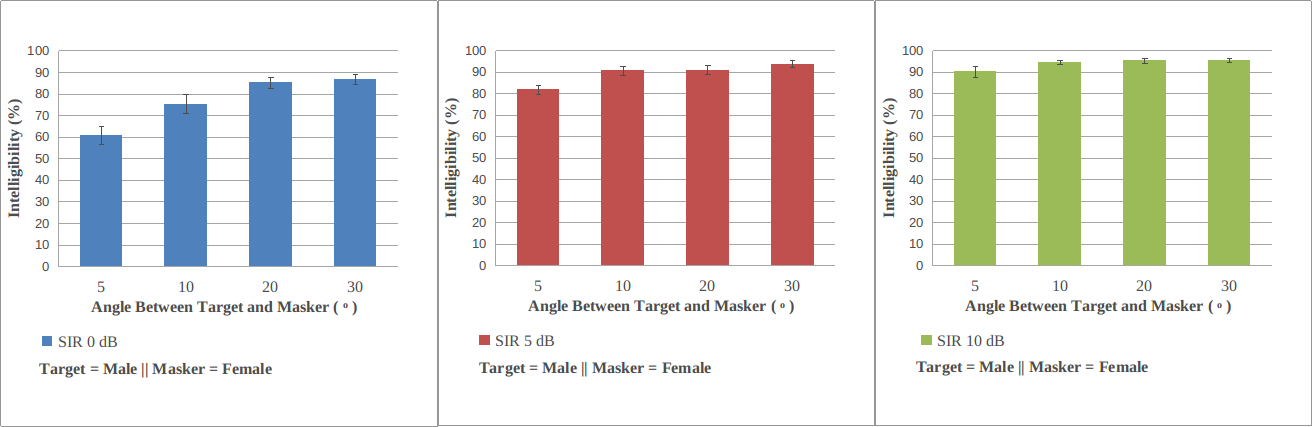
\includegraphics[scale=0.33]{../pict/pcw_mmht_fena.png}
\end{center}
\end{itemize}
\end{frame}

\begin{frame}[t]{Subjective Evaluation}
\begin{itemize}
\item Target and masker are both female speaker
\begin{center}
    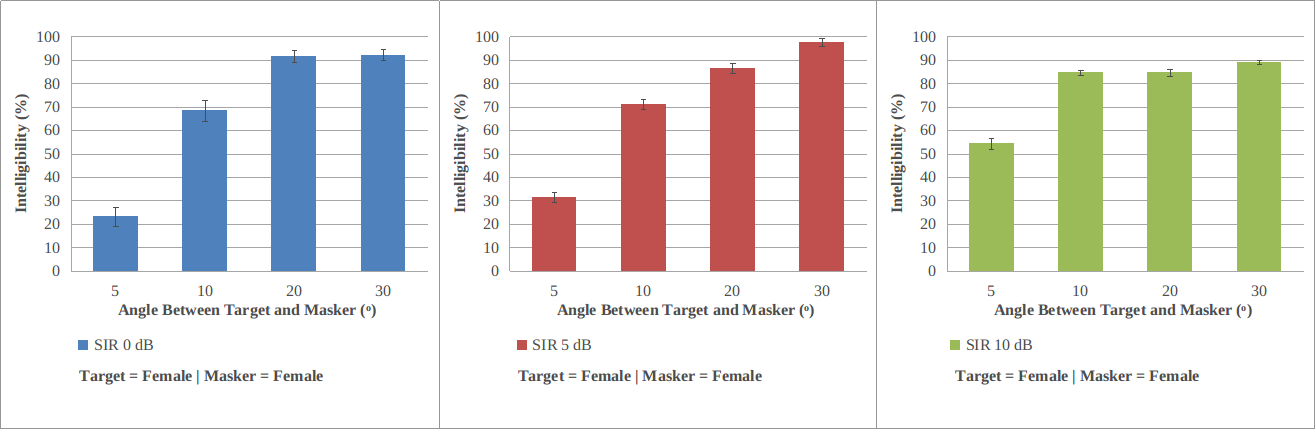
\includegraphics[scale=0.33]{../pict/pcw_fena_fena.png}
\end{center}
\end{itemize}
\end{frame}

\begin{frame}[t]{Objective Evaluation}
\begin{itemize}
\item SNR target is male speaker and masker is female speaker
\begin{center}
    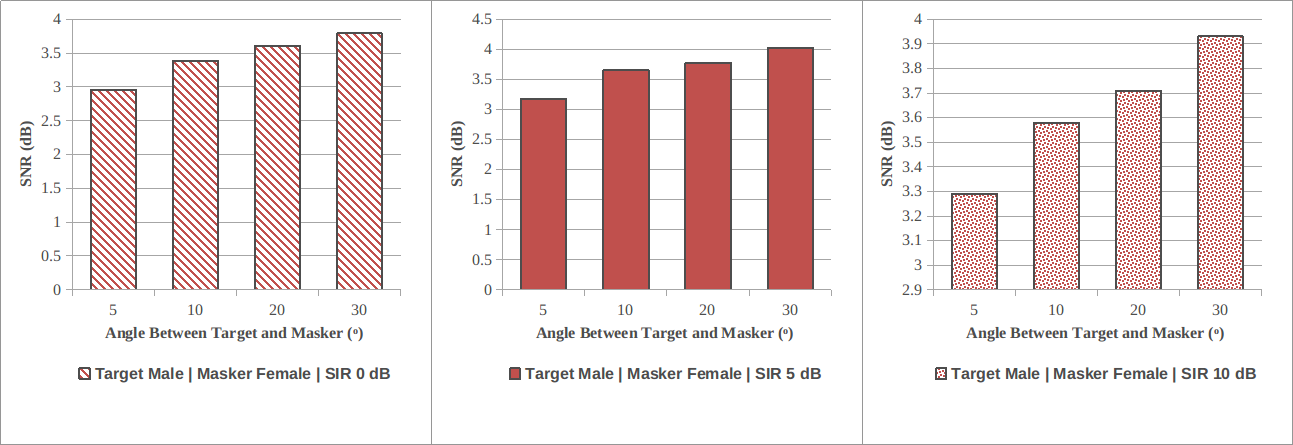
\includegraphics[scale=0.33]{../pict/snr_mmht_fena.png}
\end{center}
\end{itemize}
\end{frame}

\begin{frame}[t]{Objective Evaluation}
\begin{itemize}
\item SNR target and masker are both female speaker
\begin{center}
    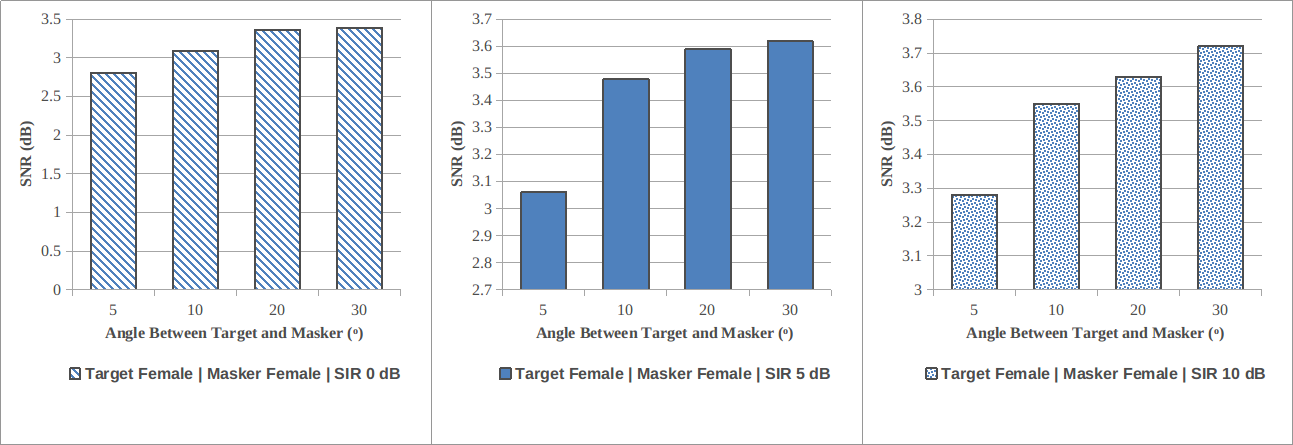
\includegraphics[scale=0.33]{../pict/snr_fena_fena.png}
\end{center}
\end{itemize}
\end{frame}

\section{Conclusion}
\begin{frame}[t]{Conclusion}
\begin{itemize}
\item Sound segregation perform well with speech intelligibility percent correct word 86\% and 3dB SNR.
\item The larger angle between target and masker then speech intelligibilty of separation result is increase.
\item The large SIR between target and masker then speech intelligibilty of separation result is increase.
\end{itemize}
\end{frame}

%%=================== CADANGAN ===================%%
%\section{Daftar Pustaka}
%\begin{frame}[t]{References}
%\bibliography{/media/linuxdata/EngineeringScience/ThesisBta/refrensi_fft_vibrasis/tesis_fft_vibrasis}
%\bibliographystyle{ieeetr}
%\end{frame}

\end{document}
